\section{Components of the HPS algorithm : Merging, Splitting and Leaf Computations}
\label{sec:quadtree}

The \gls{qahps} method applied to \refeq{eq:elliptic-pde} is broken into a factorization stage (called the build stage) and an application stage (called the solve stage). For problems in which $f(x,y)$ is non-zero, an additional ``upwards'' stage is required which handles the inhomogeneous correction.

The goal of the \gls{qahps} method is to build up a {\em solution operator set} defined as
\begin{align}
    \mathcal{S} = \{(\textbf{S}^{\tau}, \textbf{w}^{\tau}) : \ \forall\ \tau \in \mathcal{Q}_P\}
    \label{eq:solution-operator-set}
\end{align}
where \Stau and \wtau are the solution operator and the inhomogeneous correction, respectively, which can then be applied to supplied Dirichlet data \gtau such that
\begin{align}
    \textbf{u}^{\tau} = \textbf{S}^{\tau} \textbf{g}^{\tau} + \textbf{w}^{\tau},\ \forall\ \tau \in \mathcal{Q}_P.
    \label{eq:u-Sg-w}
\end{align}
Building up the solution operator set is done by successively merging child-level \gls{d2n} operators \Ttau through the computation of a Schur complement.

Each stage of the \gls{qahps} method has a leaf-level computation associated with it, as well as a 4-to-1 merge algorithm (for the build and upwards stages) or a 1-to-4 split algorithm (for the solve stage). The follows sections detail each of these in turn.

\subsection{Leaf Level Computations}
\label{sub:leaf_level_computations}

In what follows, we assume that each leaf-level quadrant in the quadtree mesh stores a uniform Cartesian grid with $M \times M$ mesh cells.  We refer to this local Cartesian mesh, along with its quadrant as a {\em patch}.  In \reffig{fig:4_to_1_patches} (left), we show four patches in a larger composite domain. Cell-centered finite difference schemes are particularly convenient for adaptively refined Cartesian meshes, since the cell-centered values are not duplicated on adjacent patches.

At the leaf-level, the build stage of the HPS methods requires the solution to a Poisson problem \eqn{elliptic-pde} discretized on an $M \times M$ cell-centered grid as
\begin{equation}
\Atau \utau = \Bctau \gtau + \ftau
\label{eq:patch_poisson_problem}
\end{equation}
where $\Bctau$ spreads Dirichlet boundary data $\gtau \in \real^{4M}$ to the grid and \ftau is the right hand side function $f(x,y)$ from \eqn{elliptic-pde} evaluated at cell centers.  We write the solution to this problem in terms of a {\em homogeneous operator} \Lhtau and an inhomogeneous operator \Linhtau which represent efficient solvers on the uniform Cartesian patch. The solution is then given by 
\begin{equation}
\utau = \Lhtau \gtau + \Linhtau \ftau
\label{eq:patch_leaf_solve}
\end{equation}
Where the context is clear, we also view operators \Lhtau and \Linhtau, boundary data \gtau and right hand side data \ftau as matrices and vectors of the appropriate sizes. The components of \utau are given by $u^\tau_{ij}$, for $i,j = 1,2,\hdots M$.  

Using these leaf-level solvers, we can now build a leaf-level DtN operator \Ttau.  In the description below, we illustrate the HPS method on the complete Poisson problem, assuming a non-zero right hand side.  We remark below, though, that if one anticipates solving for multiple right-hand sides, the build stage can be separated into a factorization stage and an "upwards" stage to handle inhomogeneous data.  

\ignore{\donna{Not sure where to put this.}  The general HPS algorithm does not specify a particular local mesh discretization, and several have been proposed in the literature.  In \citep{gillman2014direct}, the authors use a spectral collocation method and in \citep{fortunato2020ultraspherical}, a Chebyshev tensor product grid for high order finite elements was used. For compatibility with the finite volume code ForestClaw \citep{calhoun2017forestclaw}, we use a second order finite volume discretization of \refeq{eq:elliptic-pde}.}

\subsubsection{\DtN (DtN) operator}
Given a cell-centered grid solution $\utau = \Lhtau \gtau + \Linhtau \ftau$, we define ``interior" grid values $\uin \in \real^{4M}$ as those grid solution values \utau for which $i = 1$, $i = M$, $j = 1$ or $j = M$.  By analogy, components of \uout are grid solution values for which $i=0$ or $i = M+1$ or $j = 0$ or $j = M+1$.     

On a cell-centered finite volume grid, the known Dirichlet boundary values are not collocated with components of the grid solution so we discretize the Dirichlet boundary condition at the midpoint between \ukin and \ukout as
\begin{equation}
g_k^\tau = \frac{\ukout + \ukin}{2}, \quad k = 1,\hdots , 4M
\end{equation}
where $g_k$, $\ukin$ and $\ukout$ are the components of \gtau, \uin and \uout respectively.  

By analogy, we discretize Neumann data on the boundary of the patch as
\begin{equation}
v_k = \frac{\ukout - \ukin}{h}
\end{equation}
where $h$ is the mesh cell width (assumed to be uniform in both x- and y- directions).

Eliminating $\ukout$  between the two expressions, we  can express the Neumann data $v_k$ in terms of Dirichlet data $g_k$ and the interior value $\ukin$ as
\begin{equation}
v_k = \frac{2}{h}(g_k - \ukin).
\end{equation}
The vector of Neumann data on patch $\tau$ can then be expressed as 
\begin{equation}
\vtau = \frac{2}{h}(\gtau - \uin).
\end{equation}   

Introducing an operator (or a matrix of the appropriate size) \Gop that selects \uin from the grid solution data \utau, we write $\uin = \Gop \utau$ so that
\begin{equation}
\vtau = \frac{2}{h}(\gtau - \Gop (\Lhtau \gtau + \Linhtau \ftau) = 
\frac{2}{h}(I - \Gop \Lhtau)\gtau - \frac{h}{2}\Gop \Linhtau \ftau
\end{equation}
From this, we define the leaf level \DtN mapping $\Ttau \in \real^{4M \times 4M}$ as
\begin{equation}
\Ttau \equiv \frac{2}{h}(I - \Gop\Lhtau).
\label{eq:Ttau-leaf}
\end{equation}
with inhomogenenous component
\begin{equation}
\htau \equiv -\frac{2}{h}\Gop\Linhtau \ftau.
\label{eq:htau-leaf}
\end{equation}
Neumann data on the patch is then computed as
\begin{equation}
\vtau = \Ttau \gtau + \htau.
\label{eq:vtau}
\end{equation}
We refer \Ttau as a discrete \DtN operator, although the Neumann data \vtau is not the Neumann data that is commonly understood to be the result of applying a DtN map, since \vtau depends not only on the Dirichlet data \gtau, but also on the inhomogeneous data \ftau.  

\subsection{The 4-to-1 Merge Algorithm}
\label{sub:4-to-1merge}
If $\tau$ is not a leaf-level quadrant, then we construct the DtN map \Ttau {\em recursively} by merging mappings from the four children patches $\alpha$, $\beta$, $\gamma$ and $\omega$  partitioning $\tau$.  For the non-leaf, two additional operators $\Stau$ and $\Xtau$ (for non-zero $f(x,y)$) are also constructed.  Prior to this merge process, it is assumed that each patch has computed a DtN mapping \Ti, for $i=\alpha$, $\beta$, $\gamma$, $\omega$. 

\begin{figure}
    \centering
    \begin{tabular}{ccc}
        \begin{subfigure}[t]{0.3\textwidth}
            \centering
            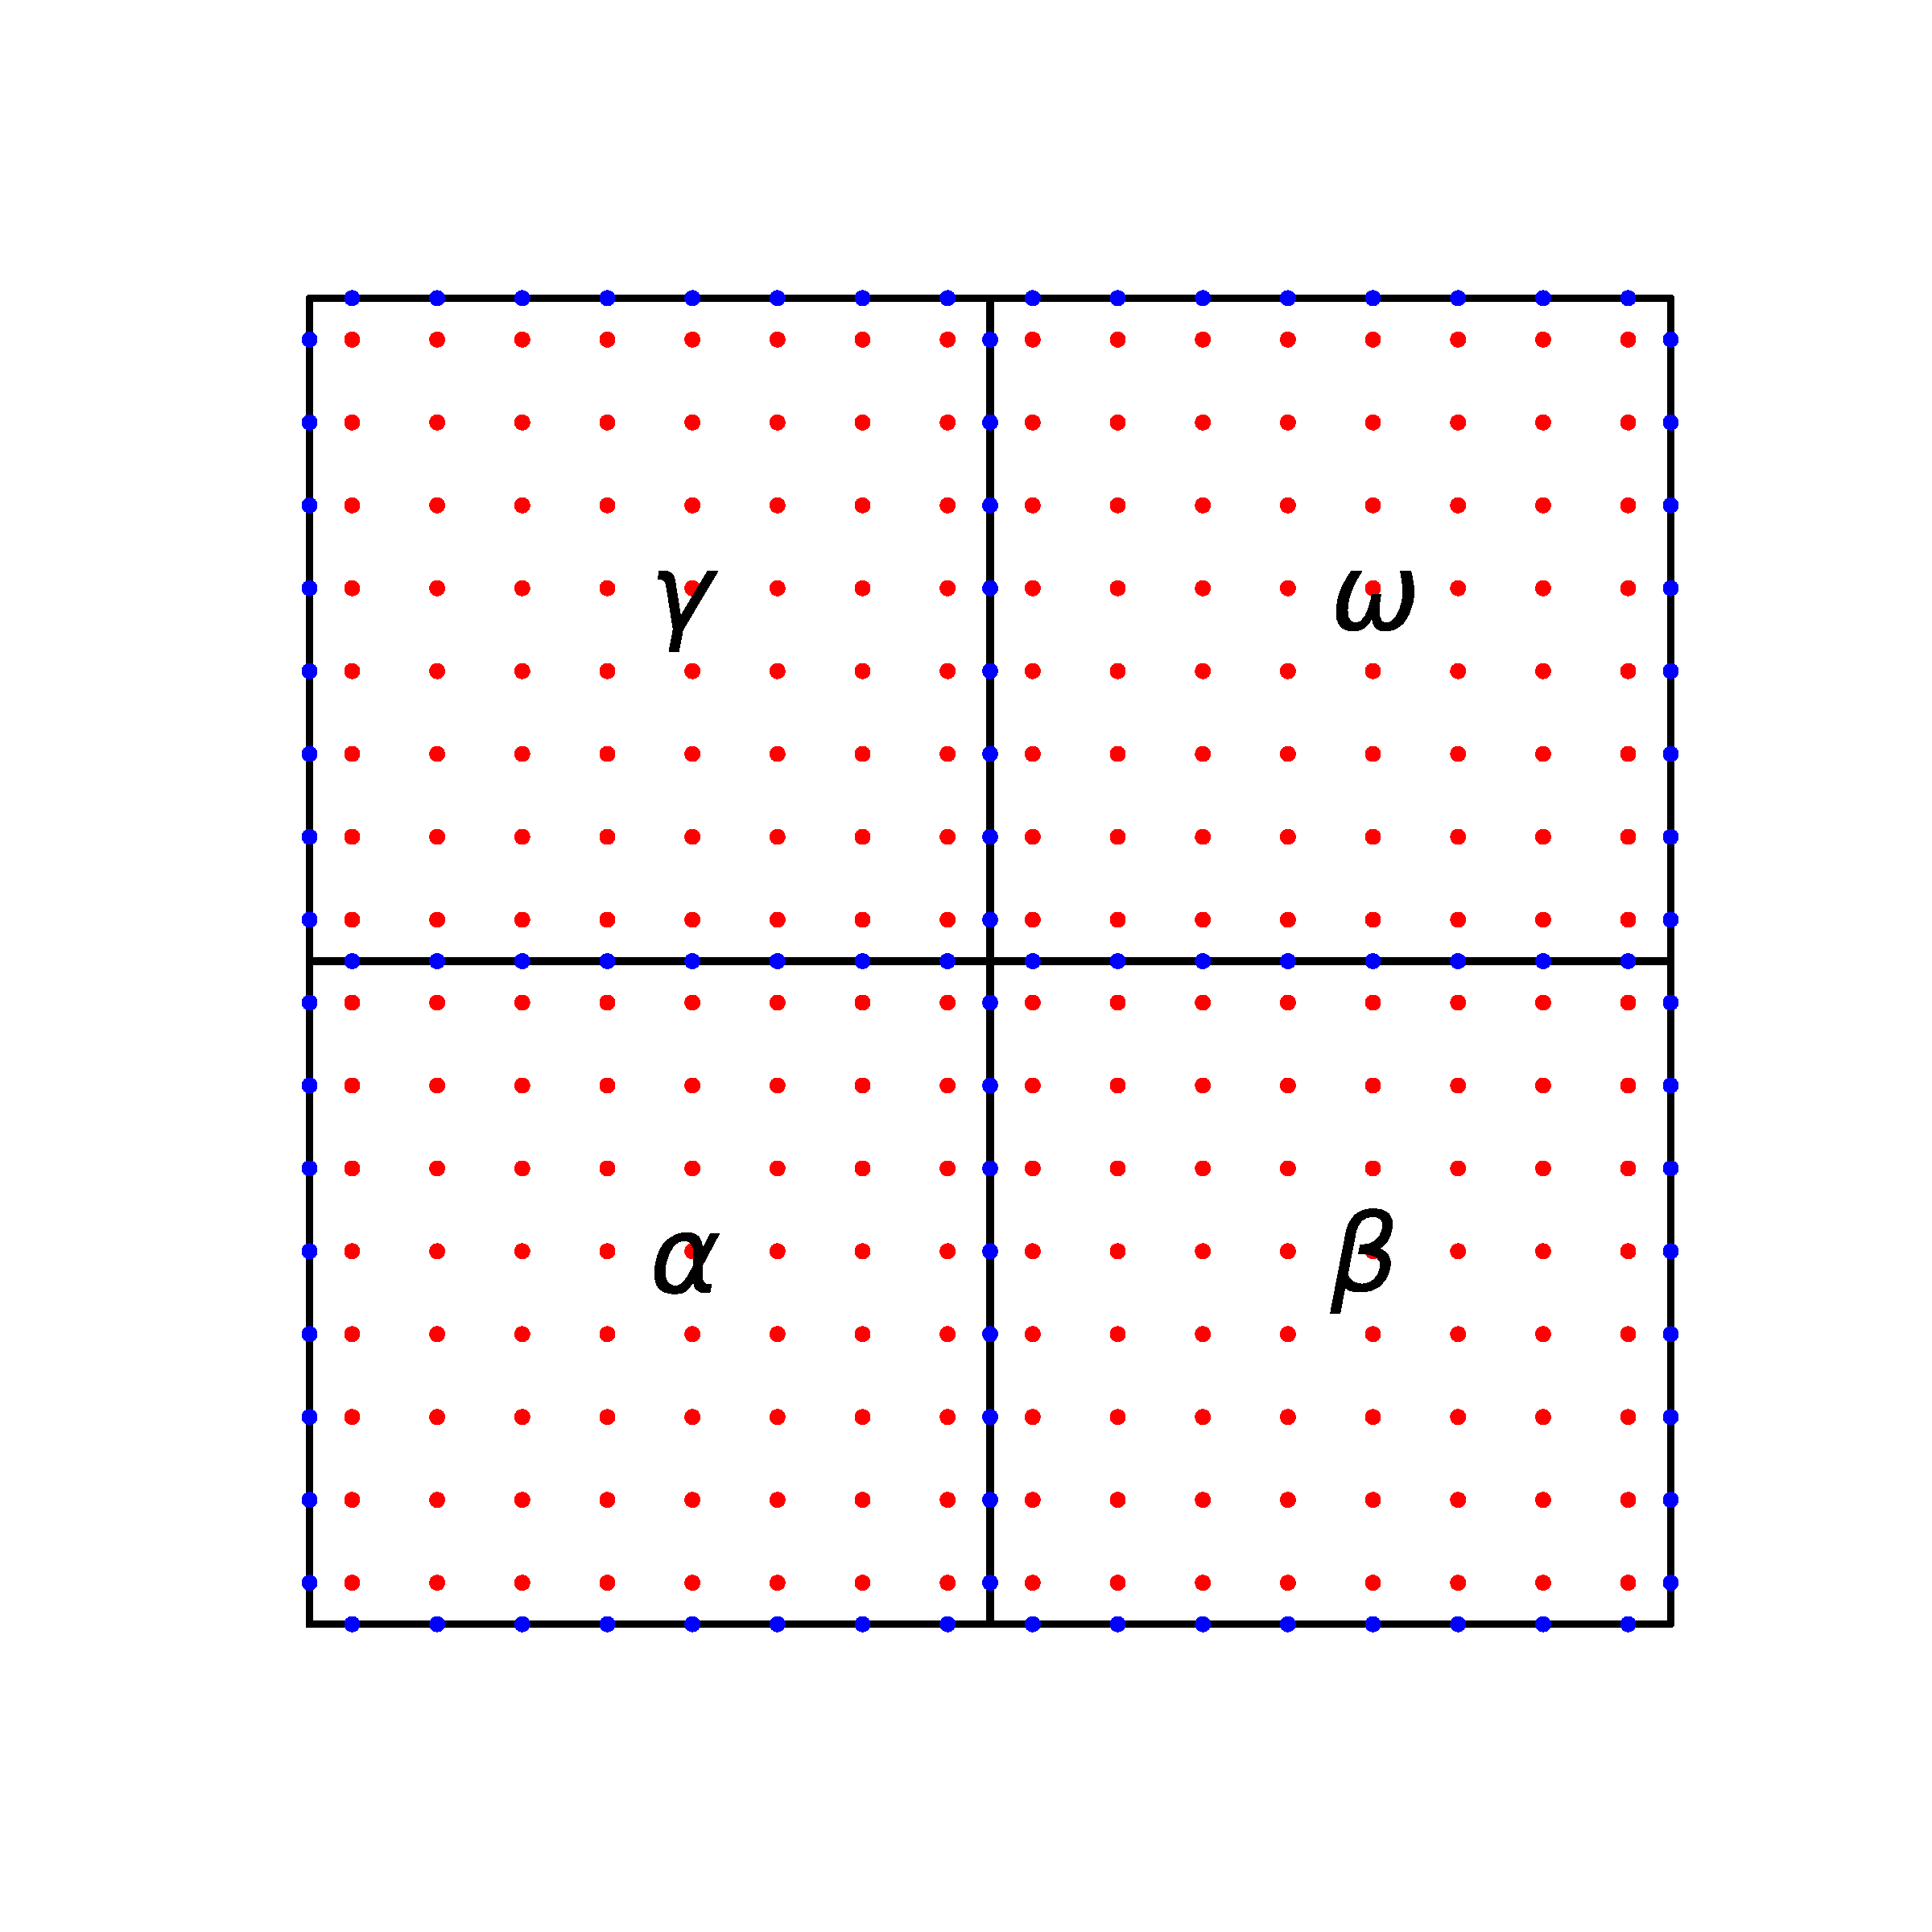
\includegraphics[width=\textwidth, clip=true, trim={100 150 100 150}]{figures/four_patches.pdf}
            \label{subfig:4_patches_with_grid}
        \end{subfigure}
        &
        \begin{subfigure}[t]{0.3\textwidth}
            \centering
            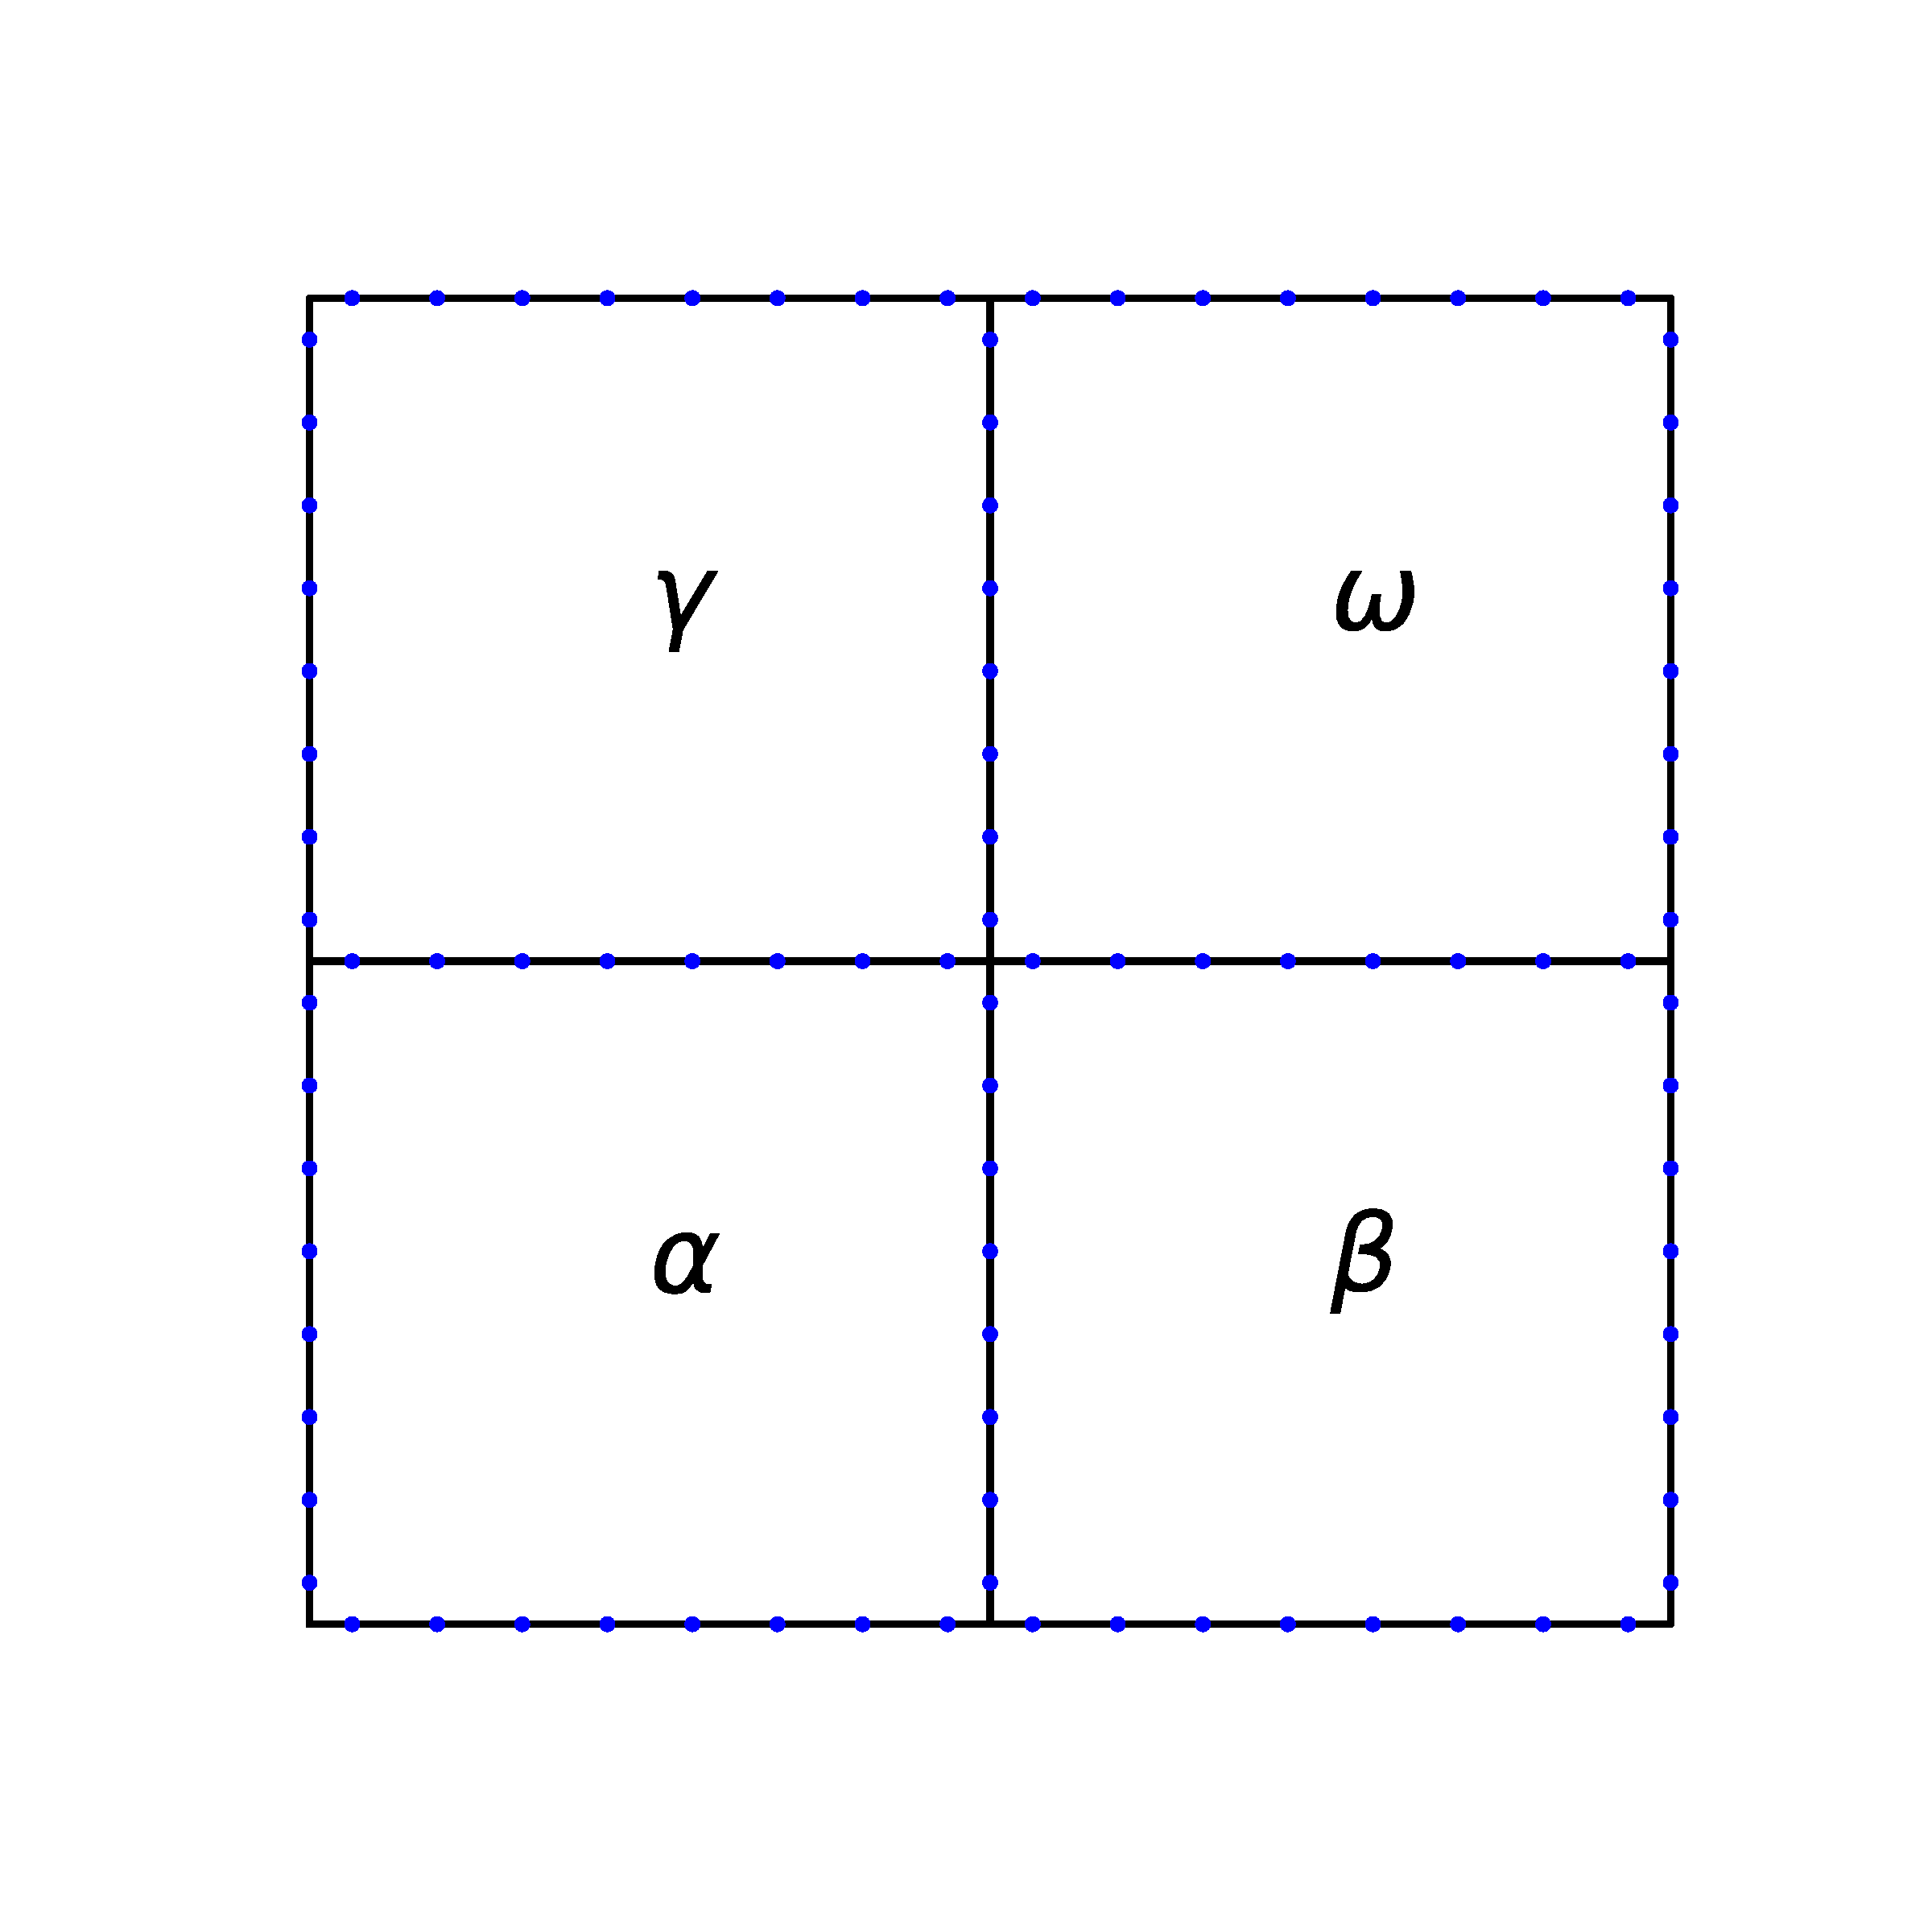
\includegraphics[width=\textwidth, clip=true, trim={100 150 100 150}]{figures/four_patches_without_points.pdf}
            \label{subfig:4_patches}
        \end{subfigure}
        &
        \begin{subfigure}[t]{0.3\textwidth}
            \centering
            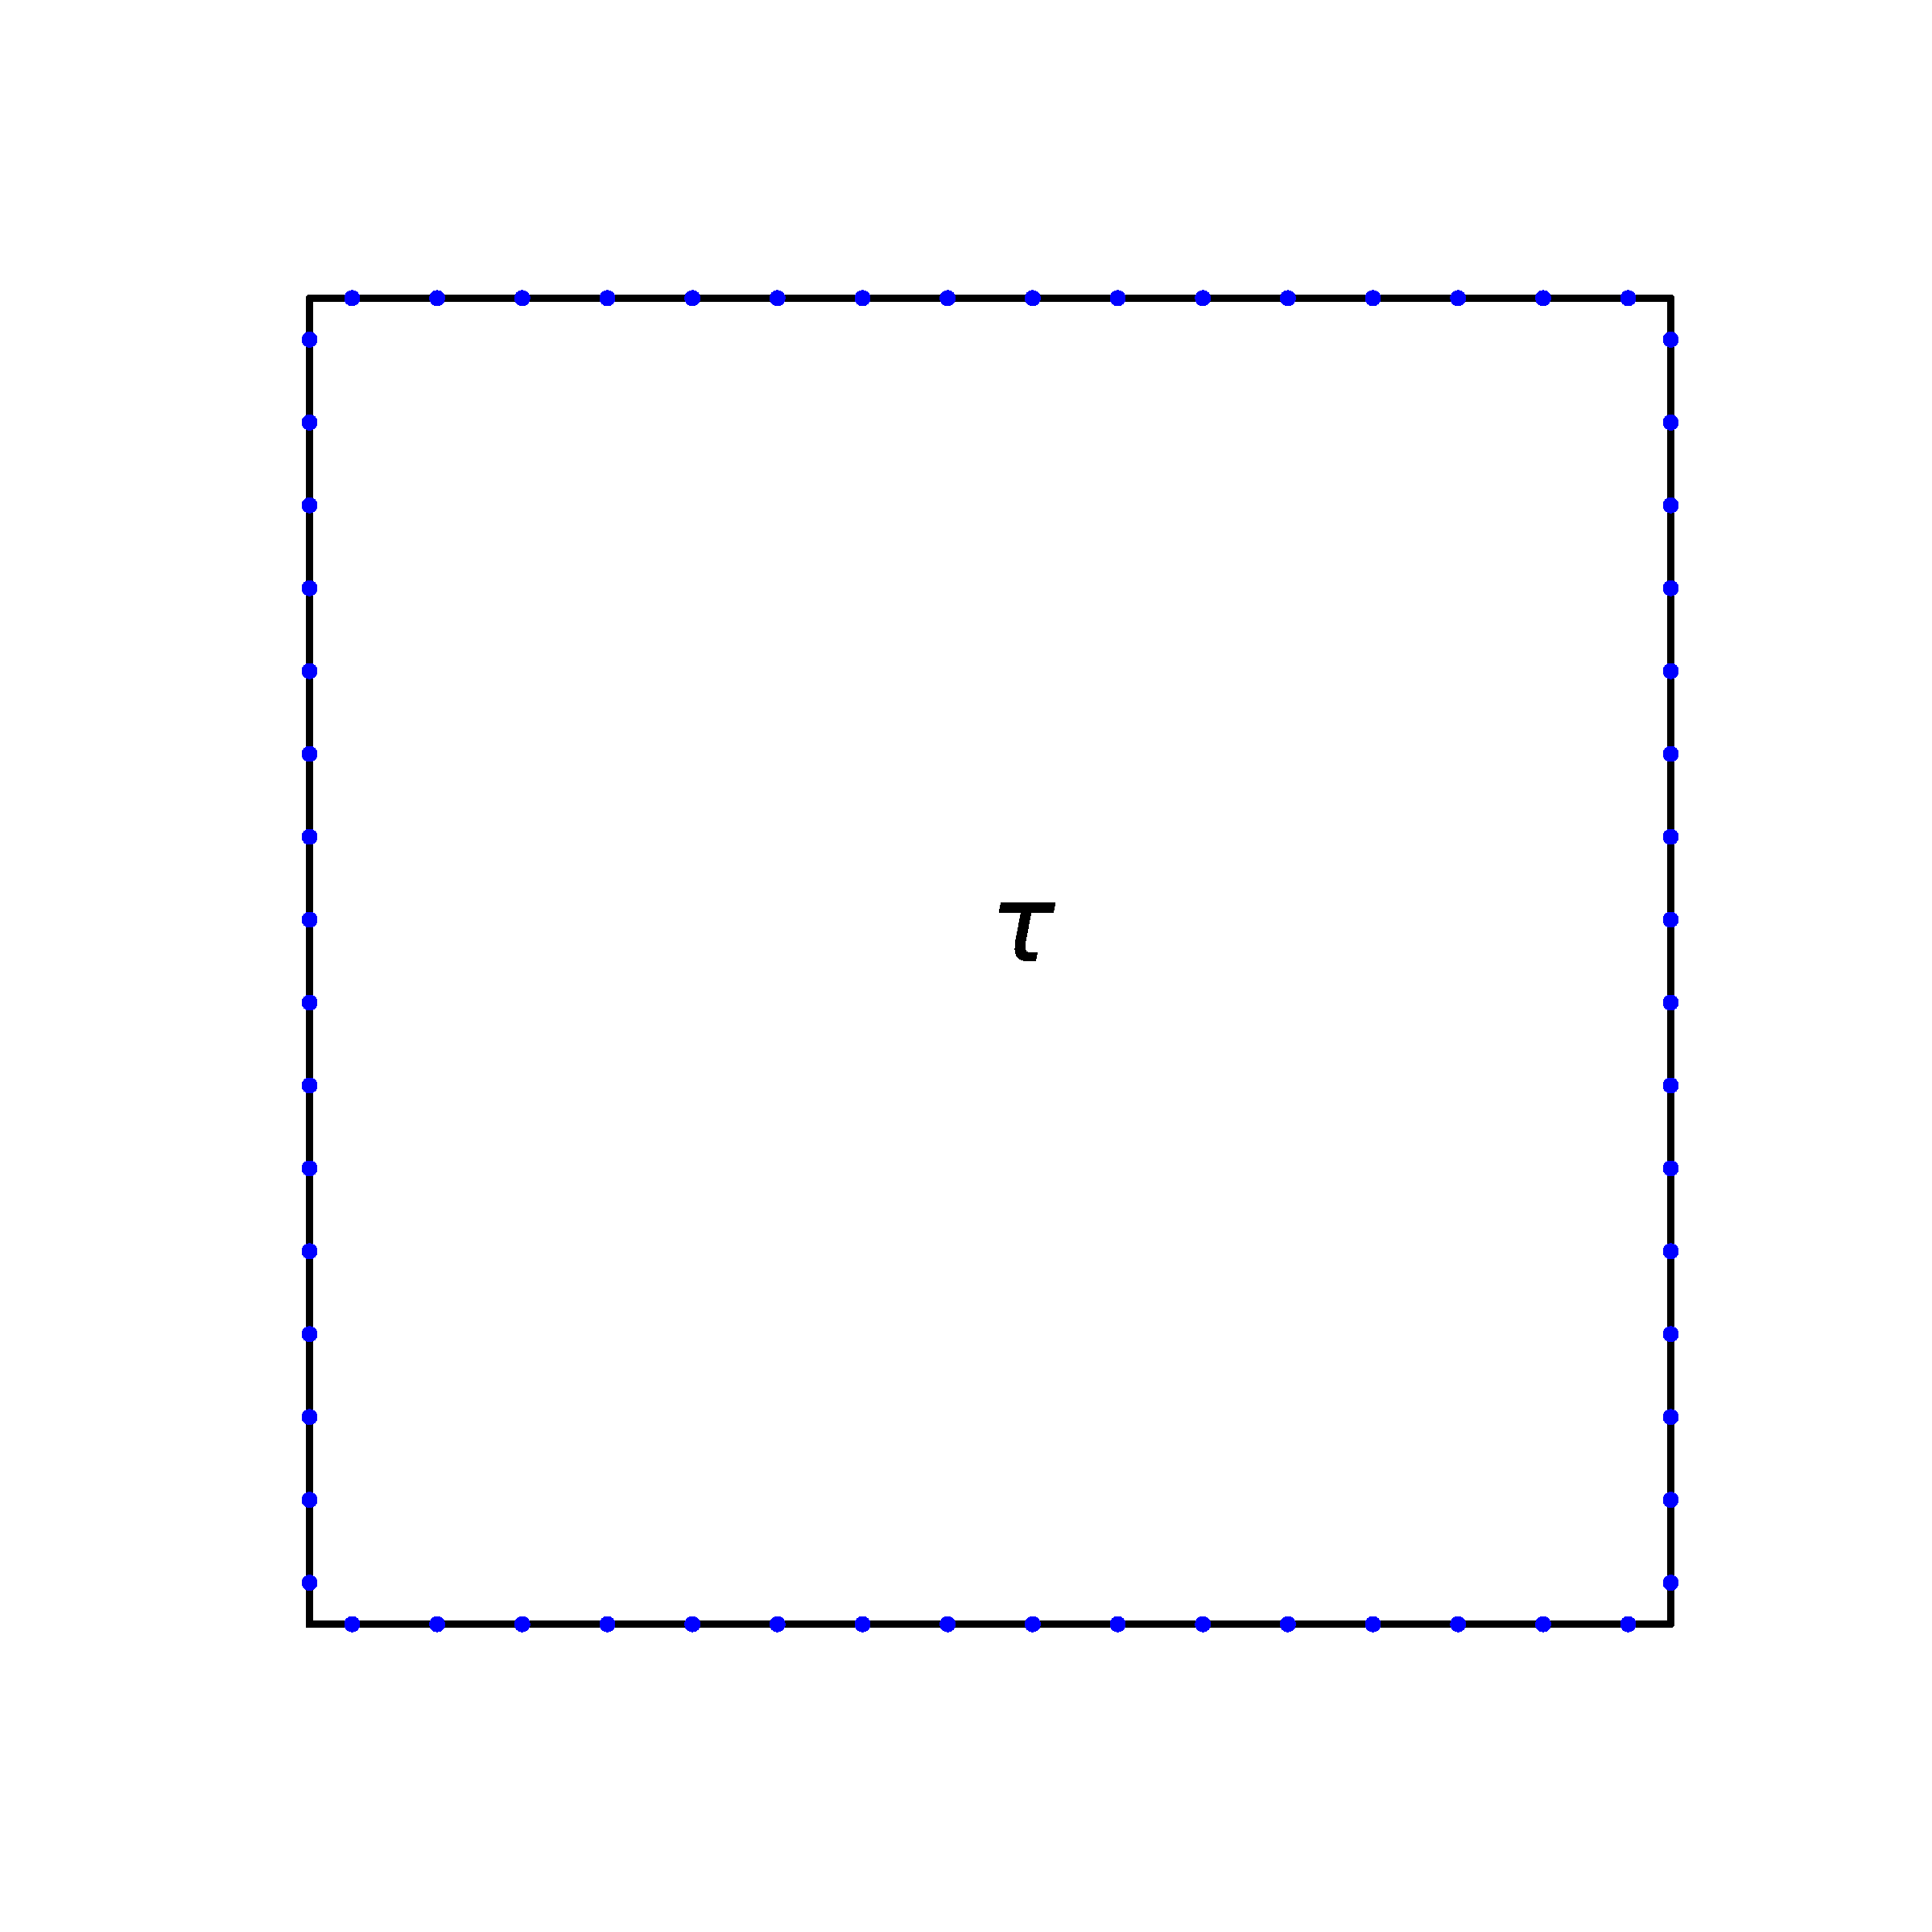
\includegraphics[width=\textwidth, clip=true, trim={100 150 100 150}]{figures/merged_patch.pdf}
            \label{subfig:parent_patch}
        \end{subfigure}
    \end{tabular}
    \caption{The 4-to-1 merge process: (left) the four children patches with their local grid, (middle) the four children share internal and external boundaries with $\tau$, (right) the merged parent patch with data on the exterior of $\tau$.}
    \label{fig:4_to_1_patches}
\end{figure}

% \begin{figure}
%     \centering
%     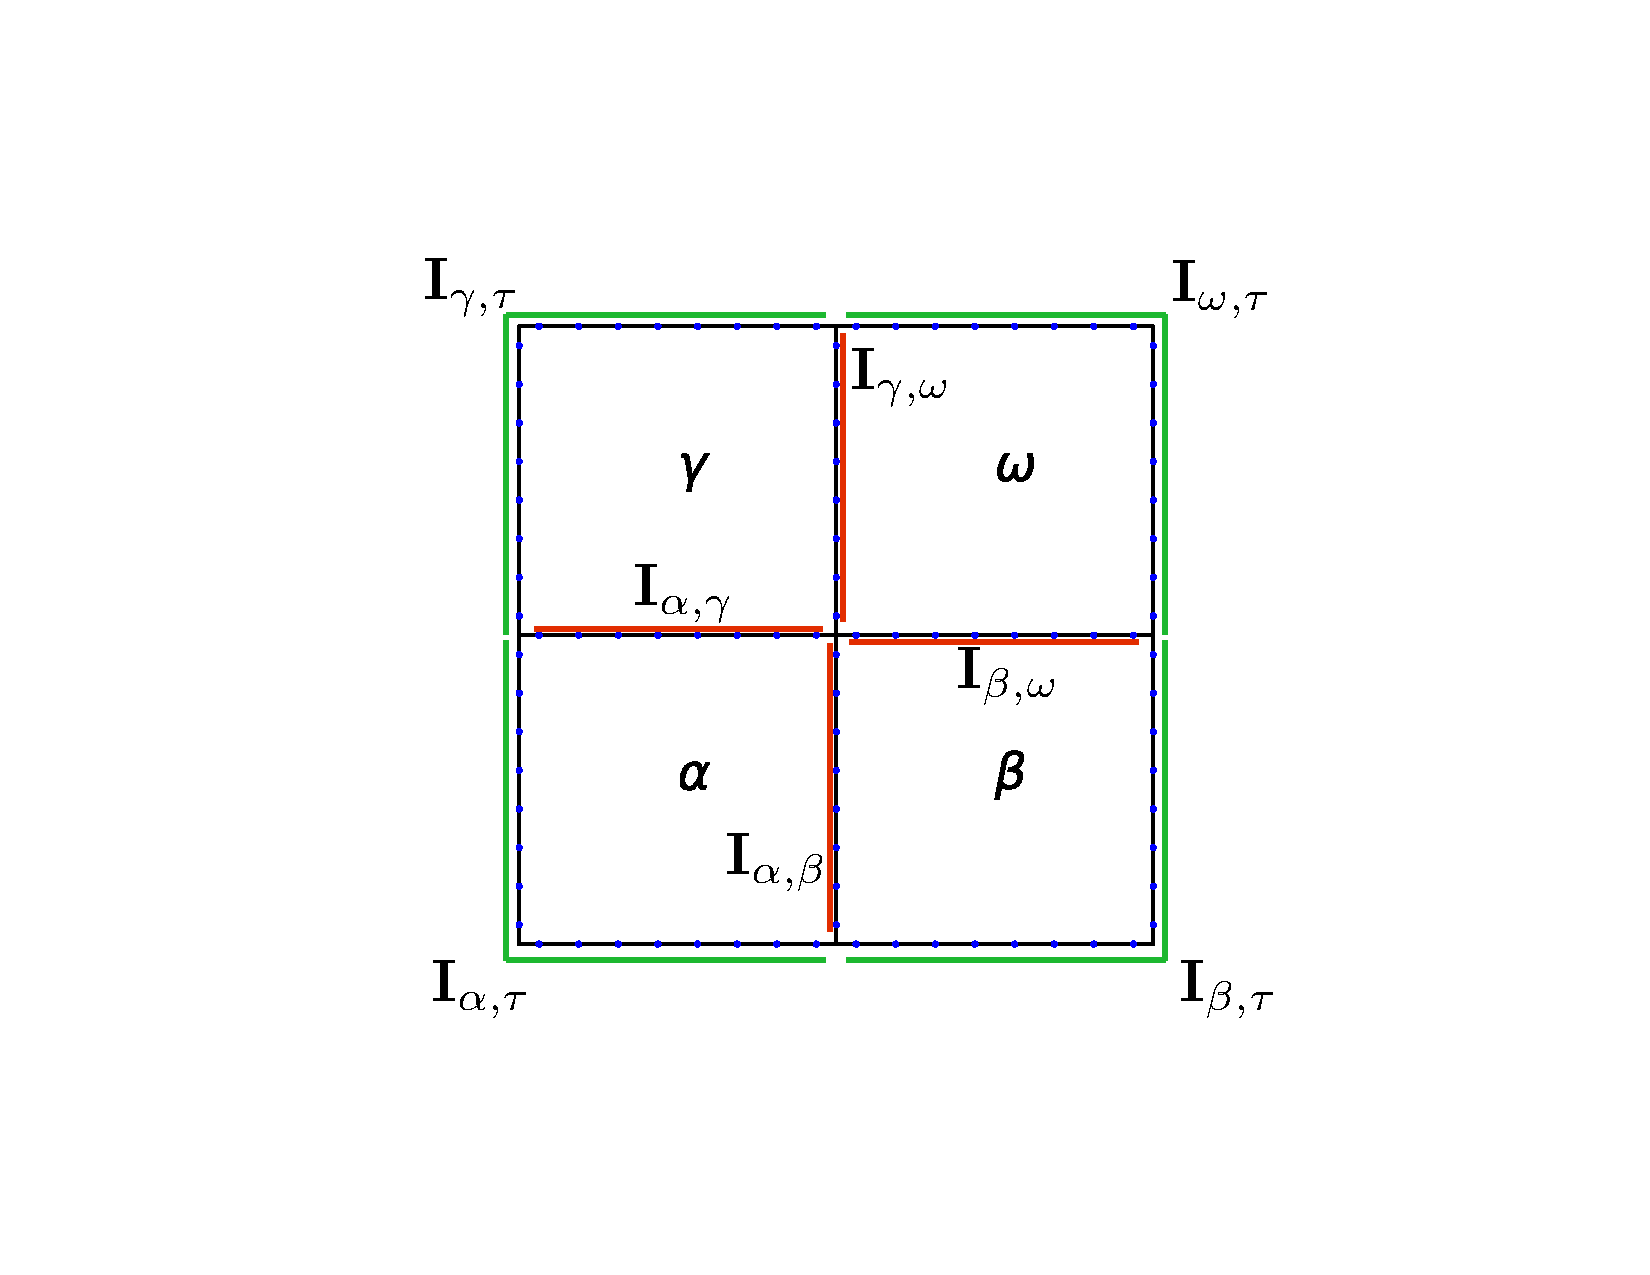
\includegraphics[width=0.5\textwidth]{figures/merging_index_sets.pdf}
%     \caption{An overview of the index sets used in the 4-to-1 merge. The index sets marked with green correspond to the exterior of $\tau$ and the index sets marked with red correspond to the interior of $\tau$.}
%     \label{fig:merged_index_sets}
% \end{figure}

\subsubsection{Merging DtN mappings} We partition sibling operators \Ti, $i=\alpha$, $\beta$, $\gamma$, $\omega$ according to how Dirichlet data on an edge of patch $i$ are mapped to an edge on $i$ containing Neumann data.  For example, the sub-matrix $\Talphap{\tau}{\gamma}$ maps Dirichlet data on the boundary shared between sibling patch $\alpha$  and parent patch $\tau$ to Neumann data on the boundary shared between patch $\alpha$ and sibling patch $\gamma$. In a similar manner, the Dirichlet data on each of the sibling patches $i$ into $\galphap{\tau}$, $\galphap{\gamma}$ and $\galphap{\beta}$, where the subscripts indicate data on edges that patch $\alpha$ shares with patches $\tau$, $\gamma$ and $\beta$. Neumann data $\valpha$ and \halpha are partitioned in an analogous manner. 

With these partitions, we can write a set of equations for each of the four sibling DtN mappings as
\begin{equation}
\begin{aligned}
\valpha = \Talpha \galpha + \halpha \quad & \Longrightarrow  & \quad 
    \begin{bmatrix}
    \valphap{\tau} \\
    \valphap{\gamma} \\
    \valphap{\beta} \\
    \end{bmatrix}
    =
    \begin{bmatrix}
    \Talphap{\tau}{\tau}   &\Talphap{\gamma}{\tau}   & \Talphap{\beta}{\tau} \\
    \Talphap{\tau}{\gamma} &\Talphap{\gamma}{\gamma} & \Talphap{\beta}{\gamma} \\
    \Talphap{\tau}{\beta}  &\Talphap{\gamma}{\beta}  & \Talphap{\beta}{\beta} \\
    \end{bmatrix}
    \begin{bmatrix}
    \galphap{\tau} \\
    \galphap{\gamma} \\
    \galphap{\beta} \\
    \end{bmatrix} + 
    \begin{bmatrix}
    \halphap{\tau} \\
    \halphap{\gamma} \\
    \halphap{\beta} \\
    \end{bmatrix}\\
&& \\
\vbeta = \Tbeta \gbeta + \hbeta \quad & \Longrightarrow  & \quad
    \begin{bmatrix}
        \vbetap{\tau} \\
        \vbetap{\omega} \\
        \vbetap{\alpha} \\
    \end{bmatrix}
    =
    \begin{bmatrix}
        \Tbetap{\tau}{\tau}   & \Tbetap{\omega}{\tau}   & \Tbetap{\alpha}{\tau} \\
        \Tbetap{\tau}{\omega} & \Tbetap{\omega}{\omega} & \Tbetap{\alpha}{\omega} \\
        \Tbetap{\tau}{\alpha} & \Tbetap{\omega}{\alpha} & \Tbetap{\alpha}{\alpha} \\
    \end{bmatrix}
    \begin{bmatrix}
        \gbetap{\tau} \\
        \gbetap{\omega} \\
        \gbetap{\alpha} \\
    \end{bmatrix} + 
    \begin{bmatrix}
        \hbetap{\tau} \\
        \hbetap{\omega} \\
        \hbetap{\alpha}
    \end{bmatrix}\\
&& \\
\vgamma = \Tgamma \ggamma + \hgamma \quad & \Longrightarrow  & \quad
    \begin{bmatrix}
        \vgammap{\tau} \\
        \vgammap{\alpha} \\
        \vgammap{\omega} \\
    \end{bmatrix}
    =
    \begin{bmatrix}
        \Tgammap{\tau}{\tau}    & \Tgammap{\alpha}{\tau}   & \Tgammap{\omega}{\tau} \\
        \Tgammap{\tau}{\alpha}  & \Tgammap{\alpha}{\alpha} & \Tgammap{\omega}{\alpha} \\
        \Tgammap{\tau}{\omega}  & \Tgammap{\alpha}{\omega} & \Tgammap{\omega}{\omega} \\
    \end{bmatrix}
    \begin{bmatrix}
        \ggammap{\tau} \\
        \ggammap{\alpha} \\
        \ggammap{\omega} \\
    \end{bmatrix} + 
    \begin{bmatrix}
        \hgammap{\tau} \\
        \hgammap{\alpha} \\
        \hgammap{\omega} \\
    \end{bmatrix}\\    
&& \\    
\vomega = \Tomega \gomega + \homega \quad & \Longrightarrow  & \quad
    \begin{bmatrix}
        \vomegap{\tau} \\
        \vomegap{\beta} \\
        \vomegap{\gamma} \\
    \end{bmatrix}
    =
    \begin{bmatrix}
        \Tomegap{\tau}{\tau}   & \Tomegap{\beta}{\tau}   & \Tomegap{\gamma}{\tau} \\
        \Tomegap{\tau}{\beta}  & \Tomegap{\beta}{\beta}  & \Tomegap{\gamma}{\beta} \\
        \Tomegap{\tau}{\gamma} & \Tomegap{\beta}{\gamma} & \Tomegap{\gamma}{\gamma} \\
    \end{bmatrix}
    \begin{bmatrix}
        \gomegap{\tau} \\
        \gomegap{\beta} \\
        \gomegap{\gamma} \\
    \end{bmatrix} +
    \begin{bmatrix}
        \gomegap{\tau} \\
        \gomegap{\beta} \\
        \gomegap{\gamma} \\
    \end{bmatrix} \\
\end{aligned}.
\label{eq:linalg_one}
\end{equation}
Taking the first equation from each of the four sets of equations in \eqn{linalg_one}, we write a system of equations for the Dirichlet data to get
\begin{equation}
A\gext + B \gint + \hext = \vext
\label{eq:sys_one}
\end{equation}
where the Dirichlet data has been partitioned into {\em exterior} data and {\em interior} data.  The exterior data is data on the boundary of the parent patch $\tau$ is given by
\begin{equation}
\gext \equiv \left[\galphap{\tau}, \gbetap{\tau} , \ggammap{\tau}, \gomegap{\tau}\right]^T
\end{equation}
To define the interior data, we use the fact that our solution is continuous across boundaries shared by sibling grids and enumerate data on the four shared boundaries as
\begin{equation}
\begin{aligned}
\gzero \equiv \galphap{\gamma} & = \ggammap{\alpha}\\
\gone \equiv \gbetap{\omega} & = \gomegap{\beta}  \\
\gtwo \equiv \galphap{\beta} & = \gbetap{\alpha} \\
\gthree \equiv \ggammap{\omega} & = \gomegap{\gamma}.
\end{aligned}
\end{equation}
With the Dirichlet data on the shared boundary uniquely defined, the interior partition of the Dirichlet data is given as
\begin{equation}
\gint \equiv \left[\gzero, \gone, \gtwo, \gthree\right]^T
\end{equation}
The Neumann data \vtau and \htau is partitioned analogously. 

The block matrices $A$ and $B$ are defined as
\begin{equation}
A = \begin{bmatrix}
\Talphap{\tau}{\tau} & \zeromat & \zeromat & \zeromat \\
\zeromat & \Tbetap{\tau}{\tau} & \zeromat & \zeromat  \\
\zeromat & \zeromat & \Tgammap{\tau}{\tau} & \zeromat  \\
\zeromat& \zeromat & \zeromat & \Tomegap{\tau}{\tau} \\
\end{bmatrix}, \qquad
B = \begin{bmatrix}
\Talphap{\gamma}{\tau} & \zeromat              & \Talphap{\beta}{\tau} & \zeromat \\
\zeromat               & \Tbetap{\omega}{\tau} & \Tbetap{\alpha}{\tau} & \zeromat \\
\Tgammap{\alpha}{\tau} & \zeromat              & \zeromat              & \Tgammap{\omega}{\tau} \\
\zeromat               & \Tomegap{\beta}{\tau} & \zeromat              & \Tomegap{\gamma}{\tau}
\end{bmatrix}
\label{eq:matrix_AB}
\end{equation}

To obtain a second set of equations, we impose a continuity condition on the normal derivative across edges shared between sibling patches and get
\begin{equation}
\begin{aligned}
\valphap{\gamma} + \vgammap{\alpha} & = \zeromat \\
\vbetap{\omega} + \vomegap{\beta} & = \zeromat \\
\valphap{\beta}  + \vbetap{\alpha} & = \zeromat\\
\vgammap{\omega} + \vomegap{\gamma} & = \zeromat.
\end{aligned}
\end{equation}
We organize the resulting four equations as
\begin{equation}
C \gext + D\gint  + \Deltah = \zeromat
\label{eq:sys_two}
\end{equation}
where
\begin{equation}
C = 
\begin{bmatrix}
\Talphap{\tau}{\gamma} & \zeromat               & \Tgammap{\tau}{\alpha} & \zeromat \\
\zeromat               & \Tbetap{\tau}{\omega}  & \zeromat                & \Tomegap{\tau}{\beta} \\ 
\Talphap{\tau}{\beta}  & \Tbetap{\tau}{\alpha} & \zeromat                & \zeromat \\
\zeromat               & \zeromat               & \Tgammap{\tau}{\omega}  & \Tomegap{\tau}{\gamma},
\end{bmatrix}
\end{equation}
\begin{equation}
D = \begin{bmatrix}
\Talphap{\gamma}{\gamma} + \Tgammap{\alpha}{\alpha} 
& \zeromat 
& \Talphap{\beta}{\gamma} 
& \Tgammap{\omega}{\alpha} \\
% 
\zeromat 
& \Tbetap{\omega}{\omega} + \Tomegap{\beta}{\beta} 
& \Tbetap{\alpha}{\omega} 
& \Tomegap{\gamma}{\beta} \\
% 
\Talphap{\gamma}{\beta} 
& \Tbetap{\omega}{\alpha} 
& \Talphap{\beta}{\beta}+ \Tbetap{\alpha}{\alpha} 
& \zeromat \\
% 
\Tgammap{\alpha}{\omega} 
& \Tomegap{\beta}{\gamma} 
& \zeromat 
& \Tgammap{\omega}{\omega} + \Tomegap{\gamma}{\gamma}
\end{bmatrix}
\label{eq:matrix_CD}.
\end{equation}
and 
\begin{equation}
\Deltah = 
\begin{bmatrix}
\halphap{\gamma} + \hgammap{\alpha} \\
\hbetap{\omega} + \homegap{\beta} \\
\halphap{\beta} + \hbetap{\alpha} \\
\hgammap{\omega} + \homegap{\gamma}
\end{bmatrix}.
\end{equation}

Combining \eqn{sys_one} and \eqn{sys_two}, we have
\begin{equation}
\begin{aligned}
A\gext + B\gint + \hext & = \vext \\
C\gext + D\gint + \Deltah & = \zeromat
\end{aligned}
\end{equation}
Writing this system as an augmented system and applying a single step of block Gaussian elimination, we get
\begin{equation}
\left[
\begin{array}{cc|c}
A & B & \vext - \hext\\
C & D & -\Deltah\\
\end{array}\right]
\;
\Longrightarrow 
\;
\left[
\begin{array}{cc|c}
A - BD^{-1}C & 0 & \vext - \hext + B D^{-1}\Deltah\\
D^{-1}C      & I & -D^{-1}\Deltah
\end{array}\right]
\label{eq:reduced_system}
\end{equation}
We express the first row of the reduced system in equation form as 
\begin{equation}
\left(A - BD^{-1}C\right) \gext = \vext - \hext + B D^{-1}\Deltah
\label{eq:complete_ops}
\end{equation}
From this, we can identify the {\em merged} DtN operator 
\begin{equation}
\Ttau \equiv \mathbf{A} - \mathbf{B} \mathbf{D}^{-1} \mathbf{C} 
\label{eq:Ttau-merged}
\end{equation}
as the operator that maps exterior Dirichlet data to exterior Neumann data, with merged inhomogeneous Neumann data given as
\begin{equation}
\htau \equiv -\hext + B D^{-1}\Deltah. 
\label{eq:htau-merged}
\end{equation}
With these choices of \Ttau and \htau  we recover the expression from \eqn{vtau}.

The second row of the reduced system \eqn{reduced_system}, given by 
\begin{equation}
\gint = -D^{-1}C \gext -D^{-1} \Deltah,
\end{equation}
shows us how to recover interior Dirichlet data \gint  from exterior data \gext.  
From this, we introduce the {\em solve} operator \Stau, given by 
\begin{equation}
\Stau \equiv -D^{-1}C
\label{eq:Stau-merged}
\end{equation}

Introducing  the operator
\begin{equation}
\Xtau \equiv -D^{-1}
\label{eq:xtau}
\end{equation}
we can write \Ttau and  \Stau in convenient form as
\begin{equation}
\begin{aligned}
\Stau & = \Xtau C \\
\Ttau & = A + B\Stau \\
\label{eq:stau_ttau}
\end{aligned}
\end{equation}
To compute the merged inhomogeneous term, we first compute
\begin{equation}
\wtau \equiv \Xtau\Deltah
\label{eq:wtau-merged}
\end{equation}
so that
\begin{equation}
\htau = -\hext - B\wtau
\label{eq:htau}
\end{equation}

Once the build stage is complete, the solve state maps Dirichlet data on parent quadrants to Dirichlet data on child quadrants via the solve operator \Stau, as
\begin{equation}
\gint = \Stau \gext + \wtau.
\label{eq:solve_eqn}
\end{equation}

The formalism presented in terms of merged components \Xtau, \Stau, \Ttau and \htau is identical to that presented in \citep{martinsson2015hierarchical} for the horizontal merge of two leaf boxes.

The build stage of HPS method is described in \Alg{build_merge_uniform}
\begin{algorithm}[H]
    \caption{Build stage on a uniformly refined quadtree mesh}
    \begin{algorithmic}[0]
        \For{$\tau = 0,1,\dots$} \Comment{Iterate over quadrants in uniform quadtree}
            \If{$\tau$ is a leaf-level patch}
                \State Build and store leaf-level DtN map \Ttau and inhomogeneous data \htau
            \Else \Comment{$\tau$ has four child patches $i$, $i=\alpha$, $\beta$, $\gamma$, $\omega$.}
                \State Solve $D\Stau = -C$ to get operator \Stau. 
                \State Build operator \Ttau using \eqn{stau_ttau}.      
                \State Solve $D\wtau = \Deltah$ using to get \wtau.  
                \State Build merged inhomogeneous vector \htau using \eqn{htau}.
                \State Store \Stau, \Ttau, \htau and \wtau with quadrant $\tau$.
                \State Delete operators \Talpha, \Tbeta, \Tgamma, \Tomega and inhomogeneous data \halpha, \hbeta, \hgamma and \homega.
            \EndIf
        \EndFor
    \end{algorithmic}
    \label{alg:build_merge_uniform}
\end{algorithm}
At the end of this build stage, we will have a single DtN operator \Ttau and single vector \htau for the root patch.  At all levels, though, we will have a solve operator \Stau and inhomogeneous vector \wtau.

A solve stage of the HPS method starts with data $g(x,y)$ defined on the boundary of the domain and successively ``splits" the domain by mapping this exterior Dirichlet data to interior data.  At the leaf level, we solve the Poisson problem \eqn{patch_poisson_problem}.  The solve stage algorithm is described in \Alg{solve_uniform}.
\begin{algorithm}[H]
    \caption{Solve stage on a uniformly refined quadtree mesh}
    \begin{algorithmic}[0]
        \For{$\tau = N,N-1,\hdots,0$} \Comment{Iterate over quadrants in uniform quadtree}
            \If{$\tau$ is a leaf-level patch}
                \State Solve patch Poisson problem \eqn{patch_poisson_problem}
            \Else{} \Comment{$\tau$ has four child patches $\alpha$, $\beta$, $\gamma$, $\omega$.}
                \State Use \eqn{solve_eqn} to map Dirichlet \gext on $\tau$ to Dirichlet data \gint on the interior shared child patch boundaries.
            \EndIf
        \EndFor
    \end{algorithmic}
    \label{alg:solve_uniform}
\end{algorithm}

% \begin{remark}
%     If the HPS solver is to be used with multiple right hand-sides for the same composite quadtree mesh, the build stage as described above should be separated into a "factorization" stage that only stores the operators \Ttau and \Stau and a second "upwards" stage that builds the inhomogeneous data \wtau from \htau for each patch. If the problem in \eqn{elliptic-pde} has zero right-hand side data, any operations involving \htau can be eliminated, since the inhomogeneous Neumann data will be identically zero.
% \end{remark}

% \remark{For a constant coefficient problem on a uniformly refined mesh, only one operator \Ttau per level needs to be computed and stored. In merge stage, this single operator can be used in place of each child patch. This significantly reduces the time needed in the build stage.}

% \remark{Neumann boundary data $v_k$ supplied along any segment of the domain boundary in \eqn{elliptic-pde} can be easily converted to a Dirichlet data $g_k$ using the formula
% \begin{equation}
% g_k = \ukin + \frac{h}{2}v_k
% \end{equation}
% This Dirichlet data is then propagated down to the leaf-level patches using \Alg{solve_uniform}.}

\subsection{Coarse-Fine Interfaces}
\label{sub:mesh_adaptivity}

The merging and splitting processes we have described so far applies only to four sibling patches occupying a coarser level quadrant. For a fully adaptive quadtree, however, not all quadrants are refined to the same level, resulting in coarse-fine interfaces (see \reffig{fig:adaptive_merge}). To accommodate for the coarse-fine interfaces, we coarsen entire patches with coarse-fine interfaces. This approach is similar to the approach used in \citep{babb2018accelerated}. The mesh is not changed as a result of this process, just the data on a patch, as detailed below.

\begin{figure}
    \centering
    \begin{tabular}{ccc}
        \begin{subfigure}[t]{0.3\textwidth}
            \centering
            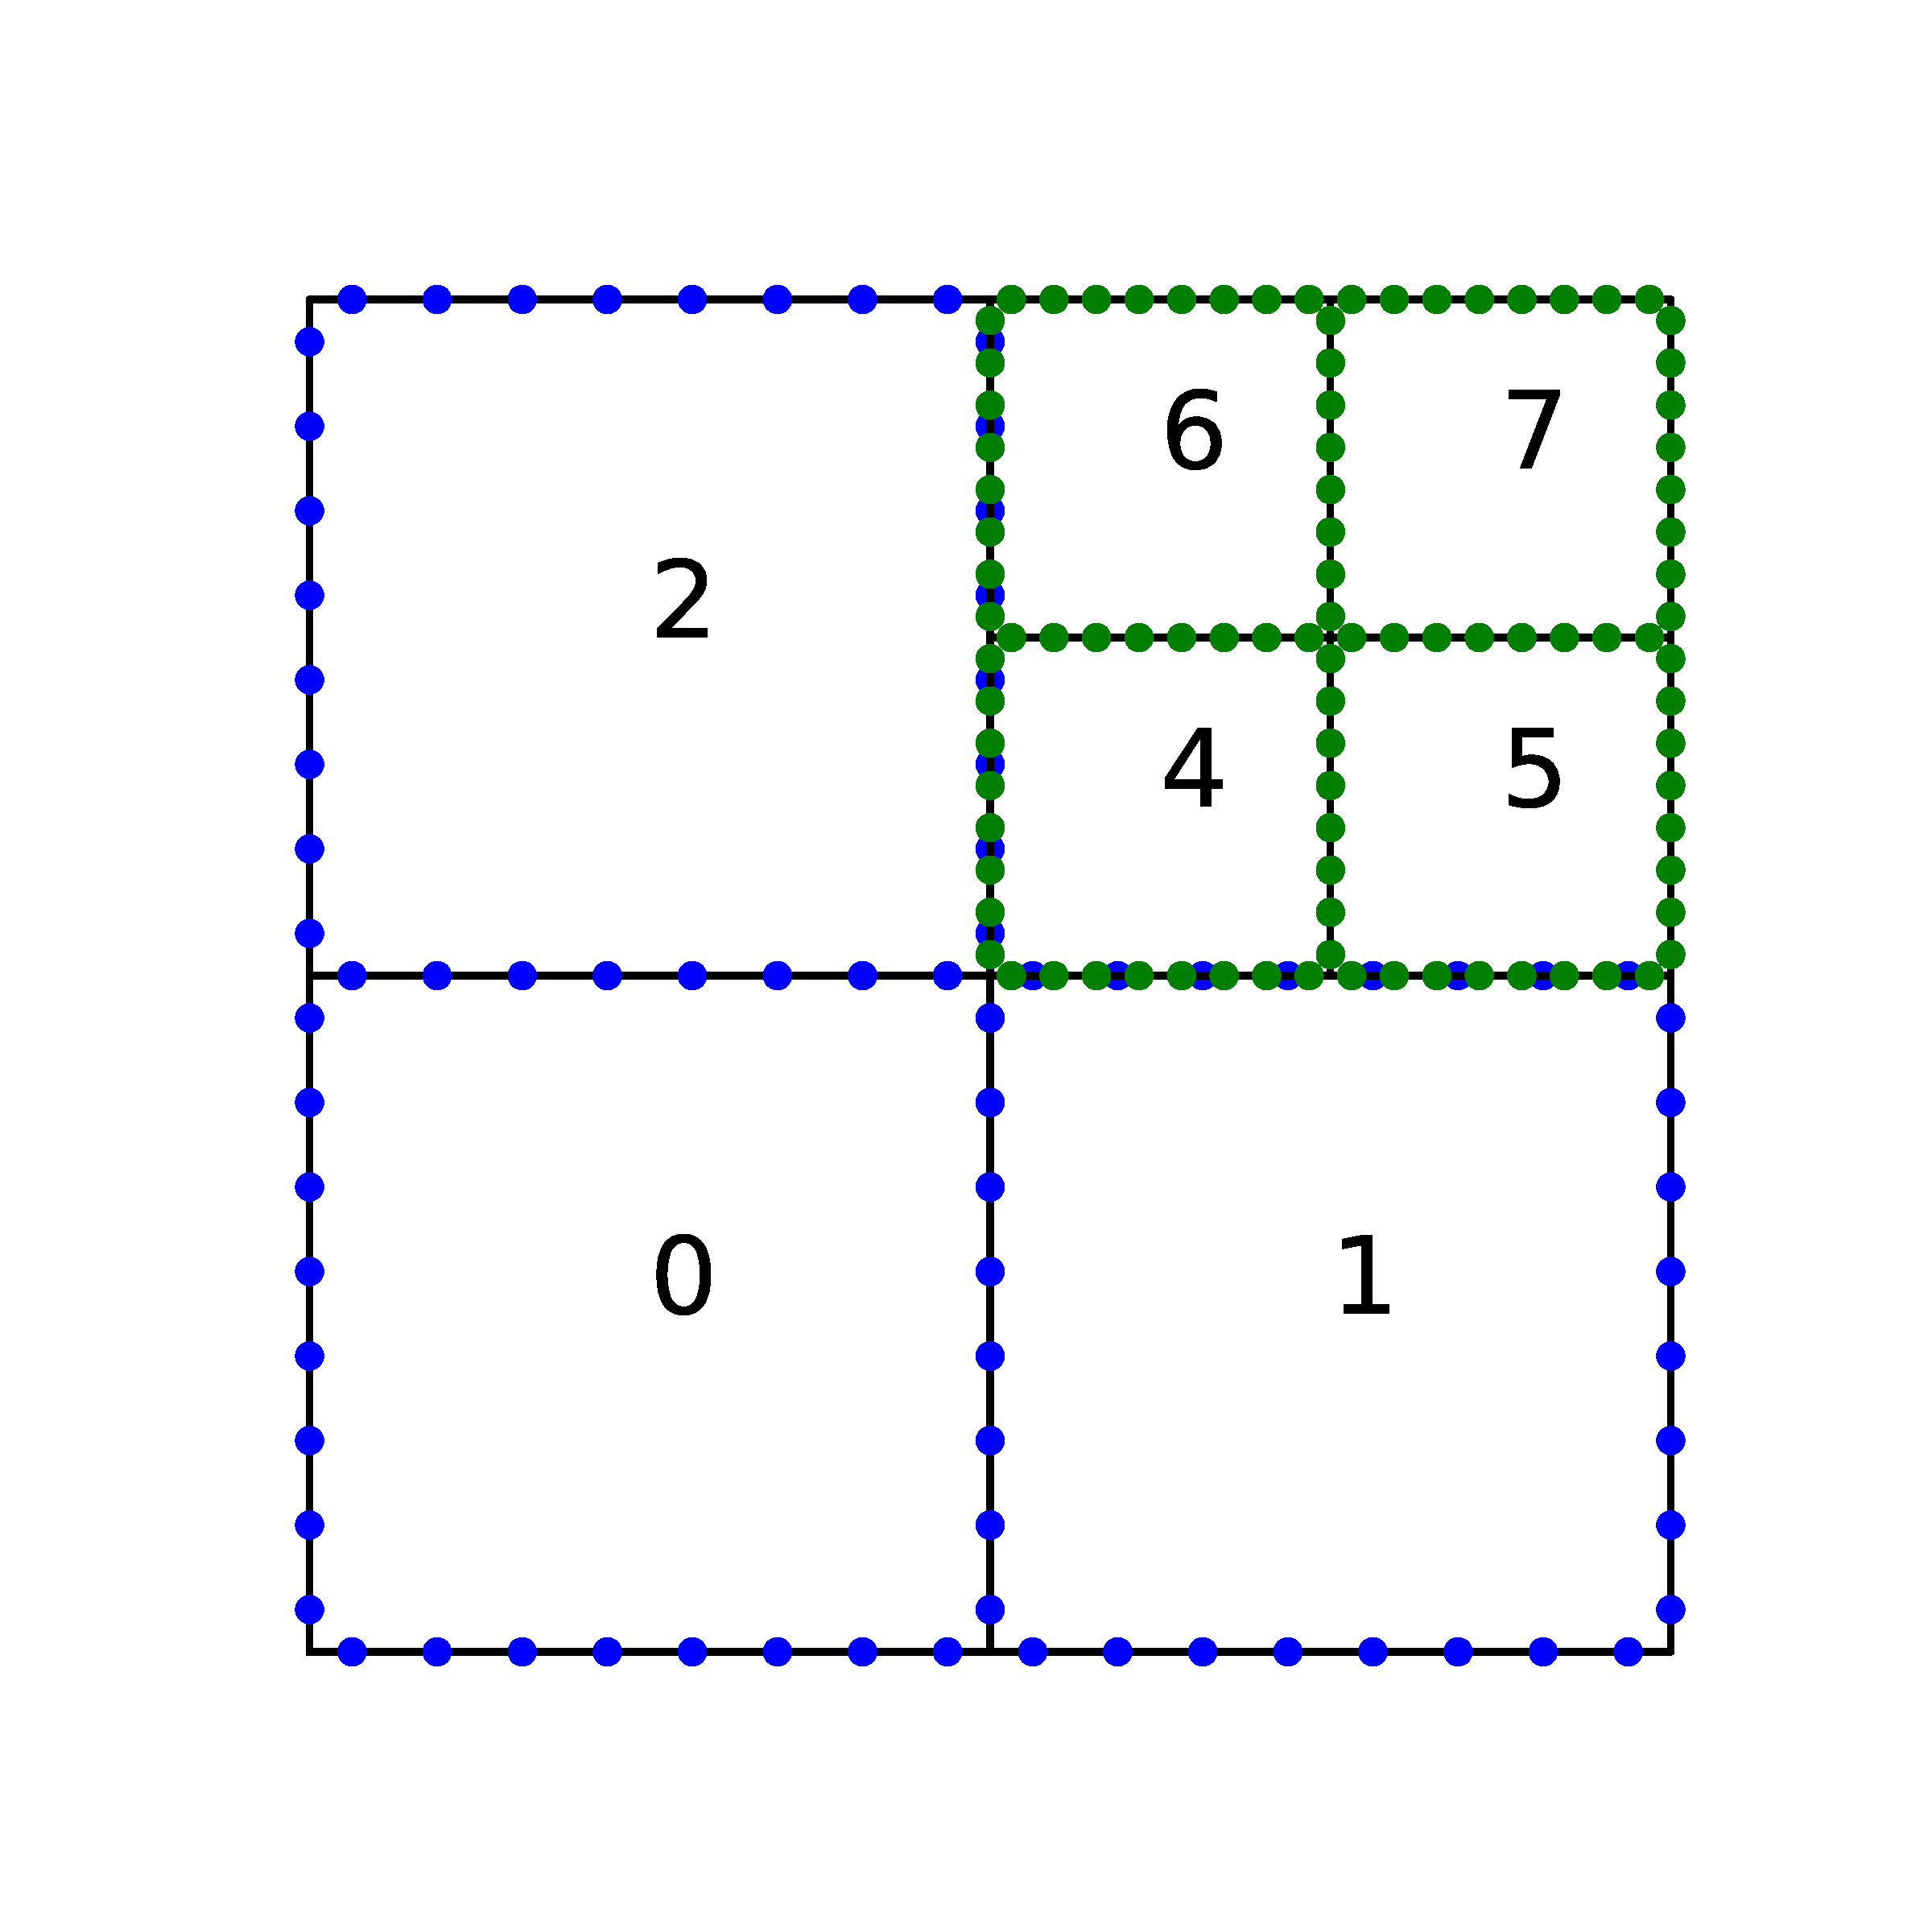
\includegraphics[width=\textwidth, clip=true, trim={100 150 100 150}]{figures/adaptive_merge1.pdf}
        \end{subfigure}
        &
        \begin{subfigure}[t]{0.3\textwidth}
            \centering
            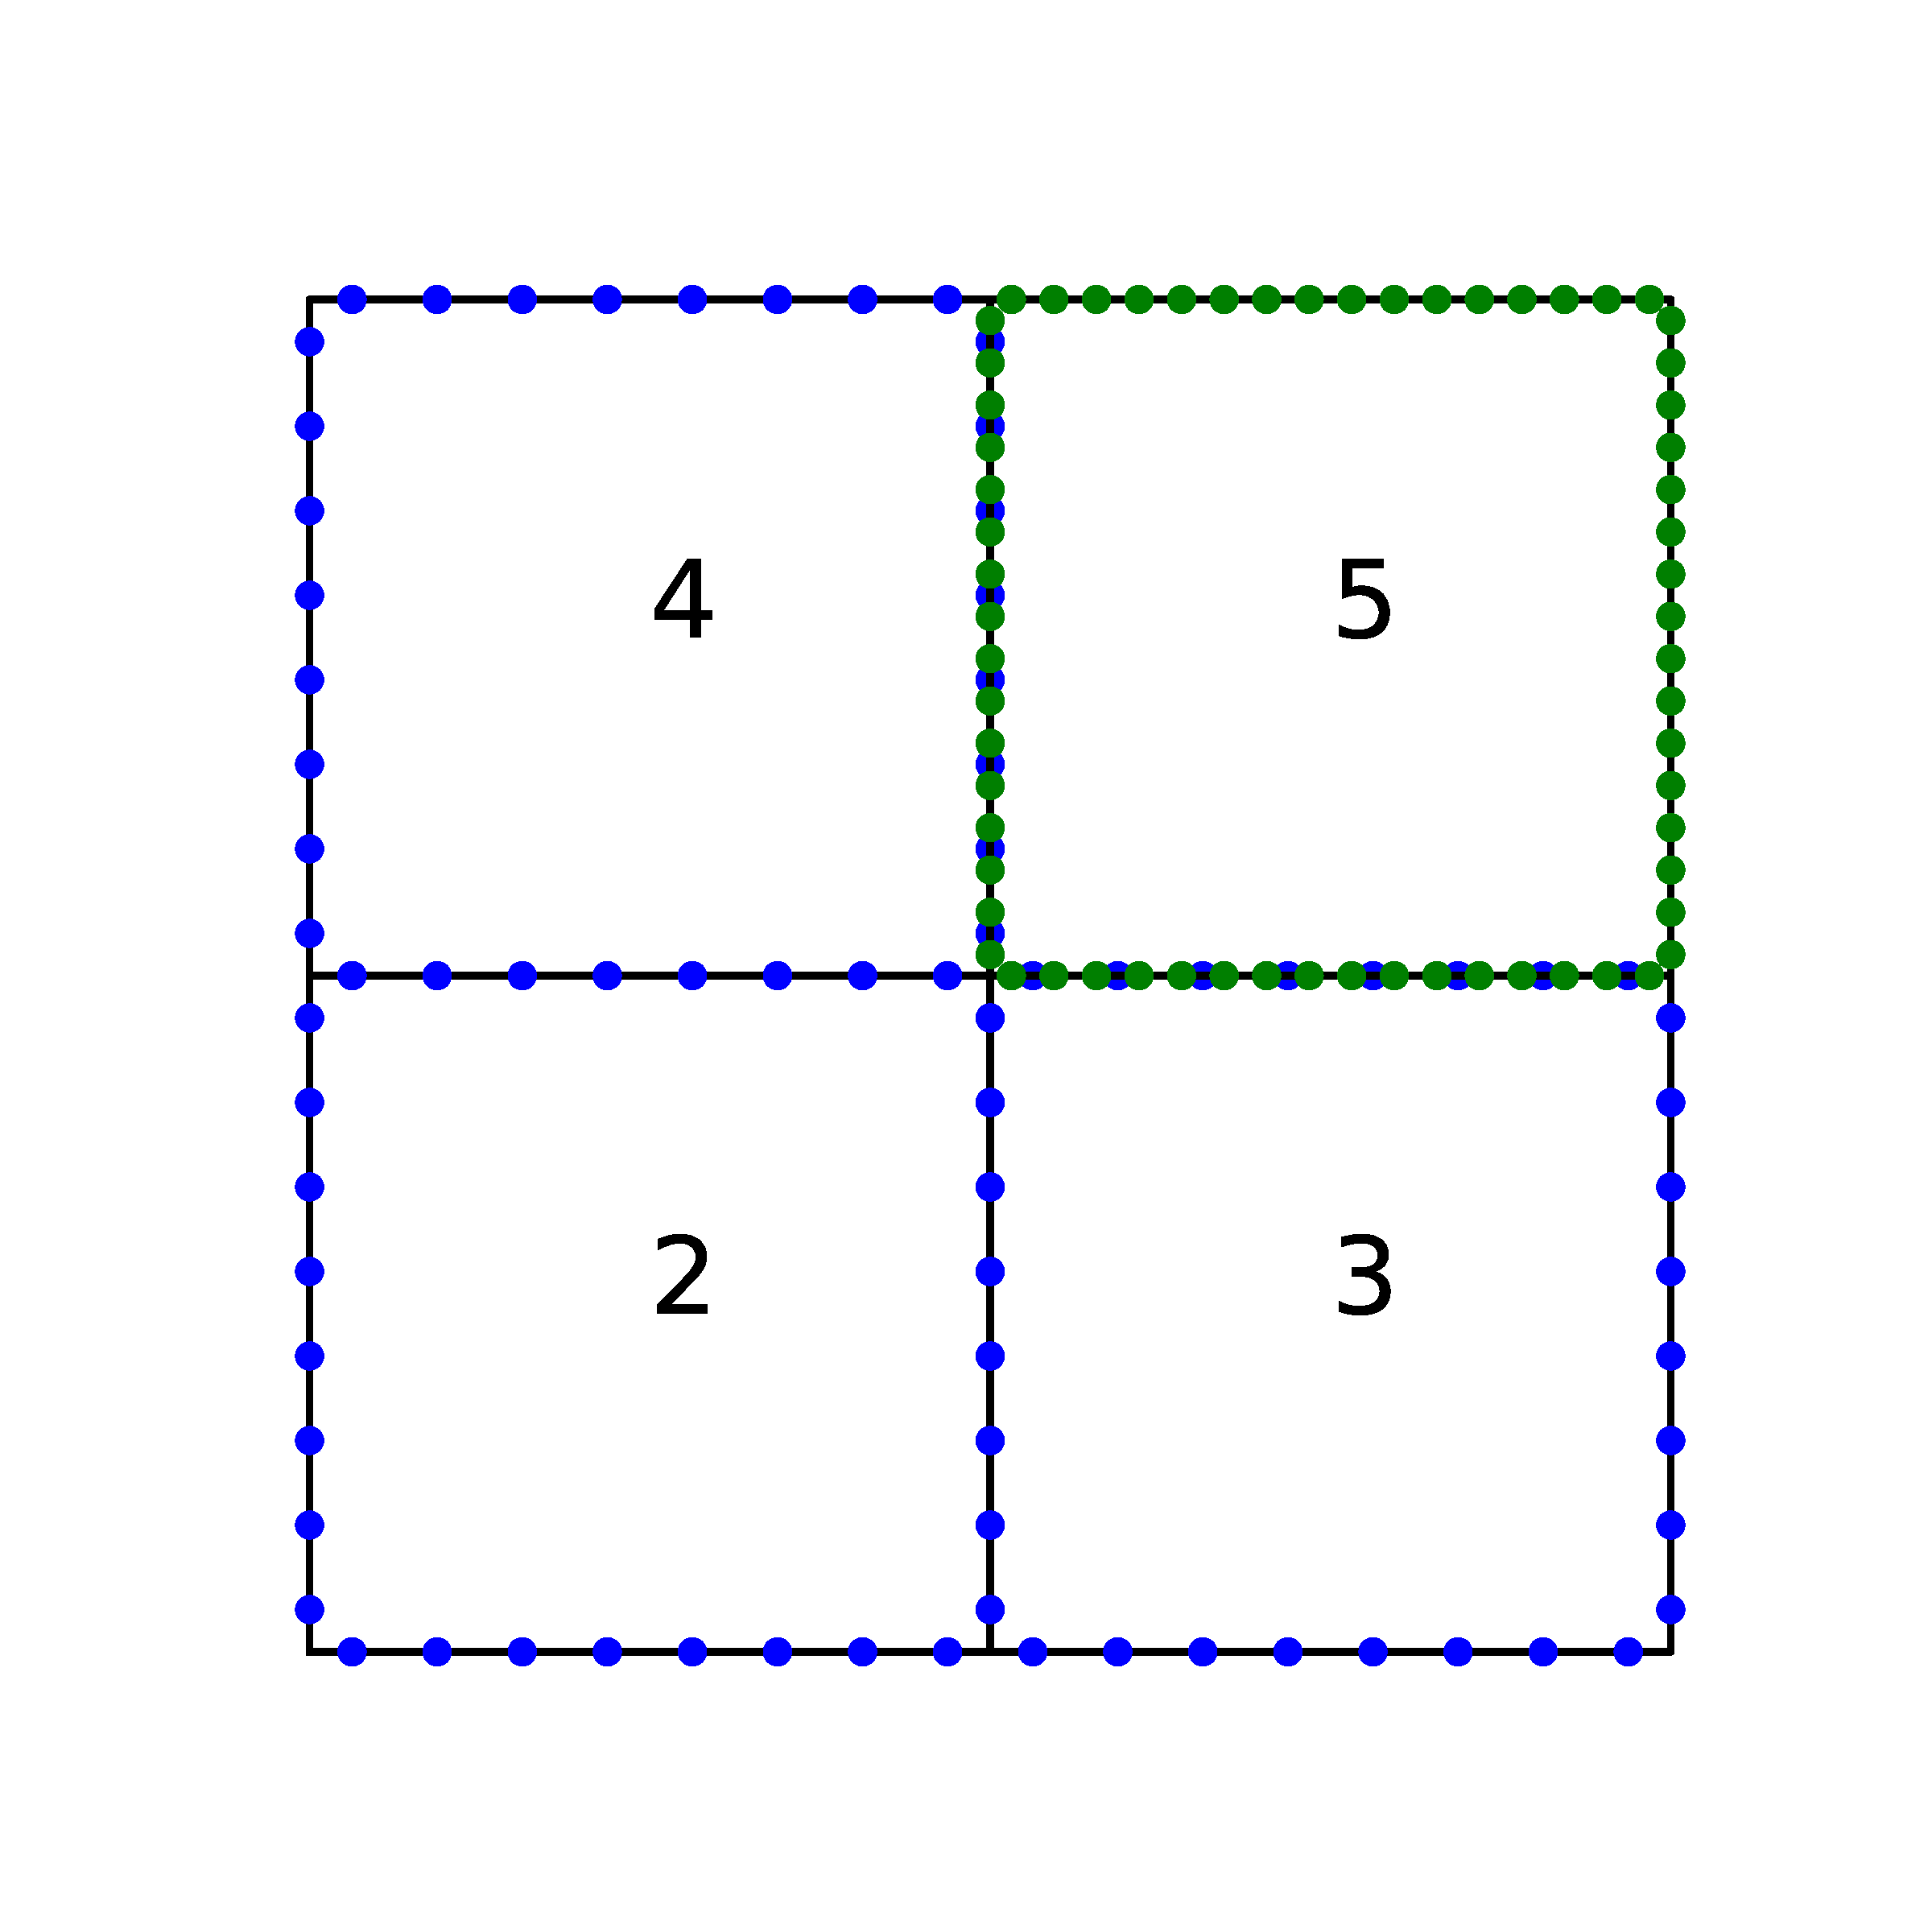
\includegraphics[width=\textwidth, clip=true, trim={100 150 100 150}]{figures/adaptive_merge2.pdf}
        \end{subfigure}
        &
        \begin{subfigure}[t]{0.3\textwidth}
            \centering
            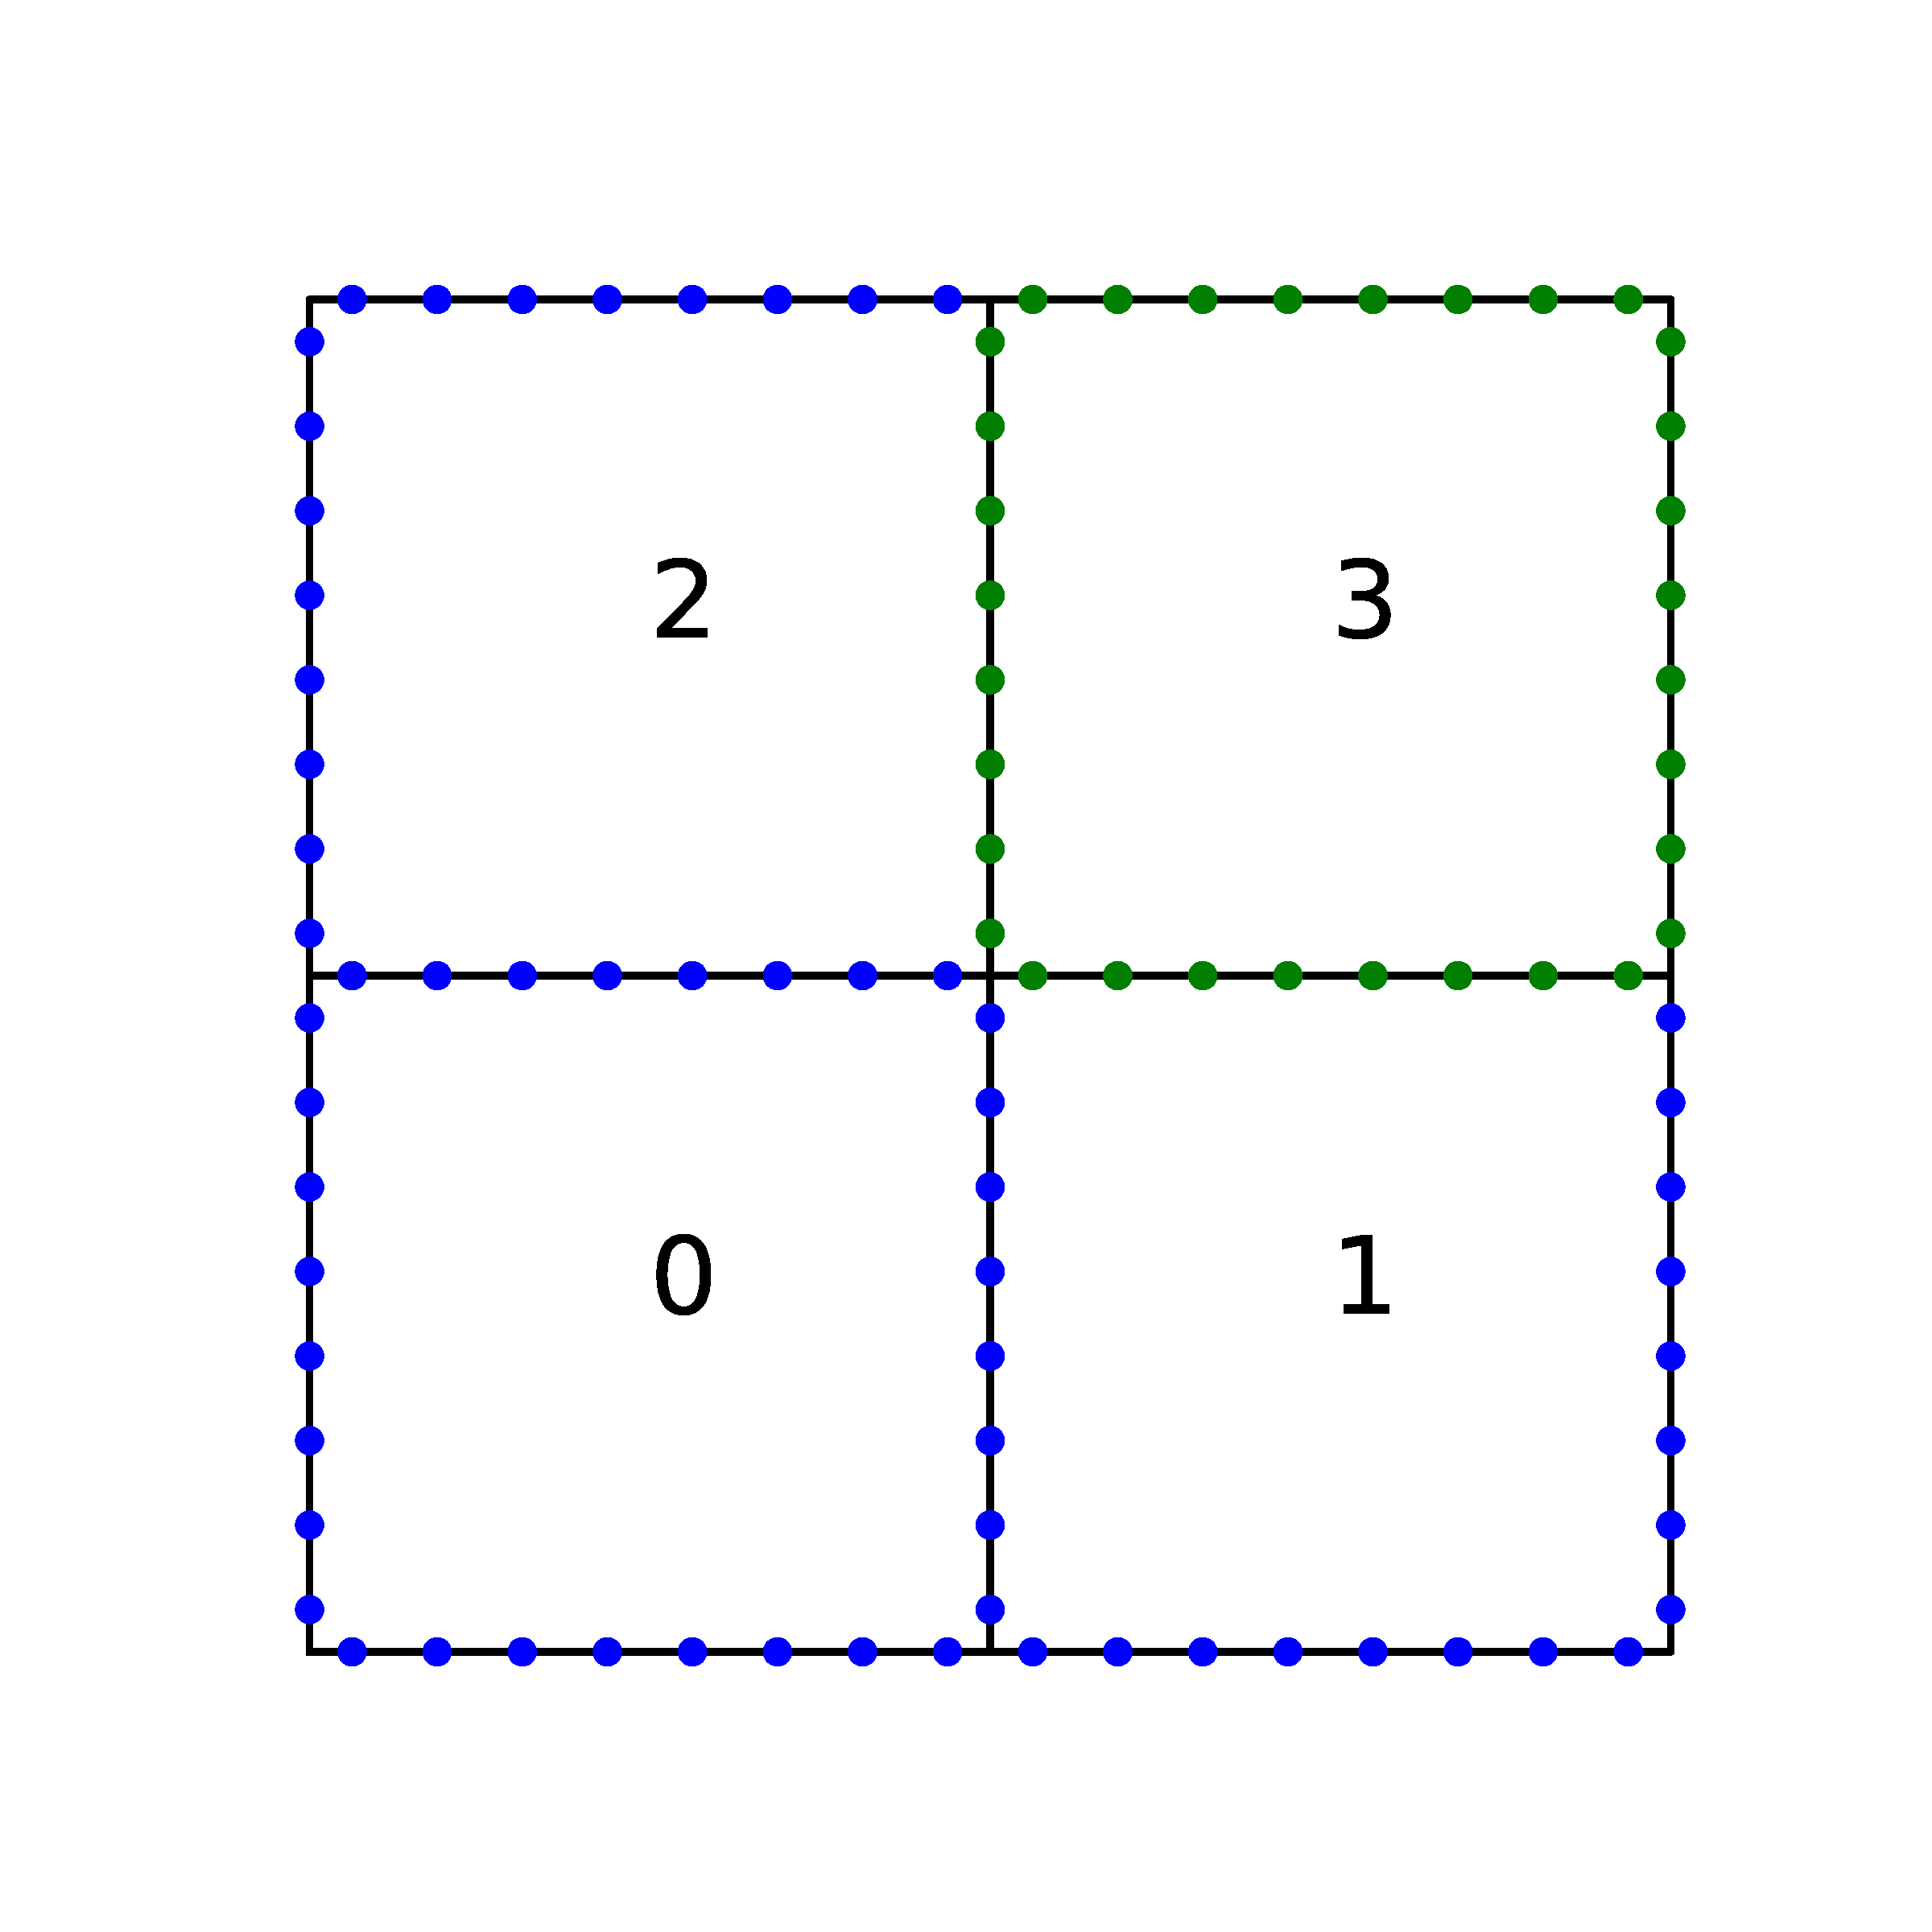
\includegraphics[width=\textwidth, clip=true, trim={100 150 100 150}]{figures/adaptive_merge3.pdf}
        \end{subfigure}
    \end{tabular}
    \caption{Example of a coarse-fine interface merge: (left) patches $6, 7, 8, \&\ 9$ will be merged and result in a coarse-fine interface, (middle) the data on patch 5 is averaged (coarsened), (right) merging $2, 3, 4, \&\ 5$ can continue as detailed in \refsec{sub:4-to-1merge}.}
    \label{fig:adaptive_merge}
\end{figure}

Prior to merging, we check each of the four children patches to be merged for a patch with data more fine than the other children. We do this by checking the size of the associated grid on that patch. If a coarse-fine interface exists, the data on that patch gets coarsened so as to match its siblings. For the build stage, only $\mathbf{T}^{\tau}$ and $\textbf{h}^{\tau}$ need to be coarsened. We form interpolation matrices $\textbf{L}_{2,1}$ and $\textbf{L}_{1,2}$ that map two sides to one or one side to two, respectively. As we employ a cell-centered grid, these matrices either average two data points to one, or interpolate one data point to two. Block diagonal versions of these are formed as
\begin{align}
    \textbf{L}_{2,1}^{B} &= \texttt{BlockDiag}(\{\textbf{L}_{2,1}, \textbf{L}_{2,1}, \textbf{L}_{2,1}, \textbf{L}_{2,1}\}) \\
    \textbf{L}_{1,2}^{B} &= \texttt{BlockDiag}(\{\textbf{L}_{1,2}, \textbf{L}_{1,2}, \textbf{L}_{1,2}, \textbf{L}_{1,2}\})
\end{align}
and coarsening $\textbf{T}$ and $\textbf{h}$ is done by matrix multiplication
\begin{align}
    \textbf{T}^{\tau'} &= \textbf{L}_{2,1}^{B} \textbf{T}^{\tau} \textbf{L}_{1,2}^{B} \\
    \textbf{h}^{\tau'} &= \textbf{L}_{2,1}^{B} \textbf{h}^{\tau}
\end{align}
where the prime indicates a coarsened version of that data.

A 1-to-4 split with a parent that has data that was coarsened during the 4-to-1 merge (for example, patch 5 from \reffig{fig:adaptive_merge}) needs to be un-coarsened. The requisite data that is un-coarsened during the solve stage is the boundary data, $\gext$ in Equation \refeq{eq:solve_eqn}. This is done with the block diagonal interpolation matrices formed above:
\begin{align}
    \textbf{g}^{\tau}_{ext} = \textbf{L}_{1,2}^{B} \textbf{g}^{\tau'}_{ext}.
\end{align}

\subsection{Comparison Between 4-to-1 Merging and 2-to-1 Merging}
\label{sub:comparison_between_4t1_and2t1_merging}

Here, we compare the performance and storage requirements for the 4-to-1 merge outlined in this paper against the 2-to-1 merge presented in \citep{gillman2014direct}. In \citep{gillman2014direct}, merging is done between two neighboring patches. To merge a family of four patches, one must do two vertical merges (merge two neighboring patches that lie next to each other in the y-direction) and then one horizontal merge (merge two ``tall-skinny'' patches that lie next to each other in the x-direction). Thus, computing and storing $\textbf{T}^{\tau}$ and $\mathbf{S}^{\tau}$ requires three, 2-to-1 merges: two vertical merges and one horizontal merge.

For both approaches, we assume that a patch has $M$ points per side, resulting in $M^2$ points per patch. We will compare the floating point operations per second (FLOPS), or FLOP count, as well as the memory needed to store the computed matrices. The merge process is seen as an elimination of the points on the interface of neighboring patches. For the 2-to-1 vertical merge, computing $\mathbf{S}$ requires $M^3$ FLOPS as a linear solve is necessary, and computing $\mathbf{T}$ requires $36M^3$ FLOPS. Storing $\mathbf{S}$ and $\mathbf{T}$ requires $6M^2$ and $36M^2$ numbers, respectively. For the 2-to-1 horizontal merge, computing $\mathbf{S}$ requires $8M^3$ FLOPS and computing $\mathbf{T}$ requires $128M^3$ FLOPS. Storing $\mathbf{S}$ and $\mathbf{T}$ requires $16M^2$ and $64M^2$ numbers, respectively. Thus, for a full 4-to-1 merge via two vertical merges and one horizontal merge, the total FLOP count is $210M^3$, with storage for $164M^2$ numbers. For the 4-to-1 merge, computing $\mathbf{S}$ requires $64M^3$ FLOPS and computing $\mathbf{T}$ requires $256M^3$ FLOPS. Storing $\mathbf{S}$ and $\mathbf{T}$ requires $32M^2$ and $64M^2$ numbers, respectively. Thus, for a 4-to-1 merge outlined in this paper, the total FLOP count is $320M^3$, with storage for $96M^2$ numbers.  Our 4-1 merge requires about 50\% more FLOPs  than a 2-1 merge on our finite volume mesh.  However, the 4-1 requires 70\% less storage.  We justify the higher FLOP count with the greater ease of implementation of the 4-1 merge over the 2-1, since only one type of merge algorithm is required.  
